\documentclass[a4paper]{article}

\usepackage[margin=1.5cm]{geometry}
\usepackage{tikz}

\pagestyle{empty}
\setlength{\parindent}{0pt}

% Grid colours
\definecolor{gridminor}{gray}{0.85}
\definecolor{gridmajor}{gray}{0.60}

% Grid line styles
\tikzset{
    axis/.style={
        black,
        line width=0.6pt
    },
    minor/.style={
        gridminor,
        line width=0.2pt
    },
    major/.style={
        gridmajor,
        line width=0.4pt
    }
}

% Cartesian grid: 0.5 cm minor spacing and 1 cm major spacing
\newcommand{\cartgrid}[4]{%
    \pgfmathtruncatemacro{\nx}{2*(#2-#1)}
    \pgfmathtruncatemacro{\ny}{2*(#4-#3)}
    \pgfmathtruncatemacro{\xmin}{ceil(#1)}
    \pgfmathtruncatemacro{\xmax}{floor(#2)}
    \pgfmathtruncatemacro{\ymin}{ceil(#3)}
    \pgfmathtruncatemacro{\ymax}{floor(#4)}

    % Minor vertical and horizontal lines
    \foreach \k in {0,...,\nx}{
        \pgfmathsetmacro{\x}{#1+0.5*\k}
        \draw[minor] (\x,#3) -- (\x,#4);
    }
    \foreach \k in {0,...,\ny}{
        \pgfmathsetmacro{\y}{#3+0.5*\k}
        \draw[minor] (#1,\y) -- (#2,\y);
    }

    % Major vertical and horizontal lines
    \foreach \x in {\xmin,...,\xmax}{
        \draw[major] (\x,#3) -- (\x,#4);
    }
    \foreach \y in {\ymin,...,\ymax}{
        \draw[major] (#1,\y) -- (#2,\y);
    }
}

% Polar grid: 0.5 cm minor circles and 15 degree minor rays;
% 1 cm major circles and 30 degree major rays
\newcommand{\polargrid}[3]{%
    \pgfmathtruncatemacro{\nminor}{(#3-#2)/15}
    \pgfmathtruncatemacro{\nmajor}{(#3-#2)/30}
    \pgfmathtruncatemacro{\nradii}{2*#1}

    % Minor radial lines
    \foreach \k in {0,...,\nminor}{
        \pgfmathsetmacro{\theta}{#2+15*\k}
        \draw[minor] (0,0) -- (\theta:#1);
    }

    % Major radial lines
    \foreach \k in {0,...,\nmajor}{
        \pgfmathsetmacro{\theta}{#2+30*\k}
        \draw[major] (0,0) -- (\theta:#1);
    }

    % Minor concentric circles
    \foreach \k in {1,...,\nradii}{
        \pgfmathsetmacro{\r}{0.5*\k}
        \draw[minor] (#2:\r) arc[start angle=#2,end angle=#3,radius=\r];
    }

    % Major concentric circles
    \foreach \r in {1,...,#1}{
        \draw[major] (#2:\r) arc[start angle=#2,end angle=#3,radius=\r];
    }
}

\begin{document}

% Page 1: Full plane

\vspace*{\fill}

\begin{center}
    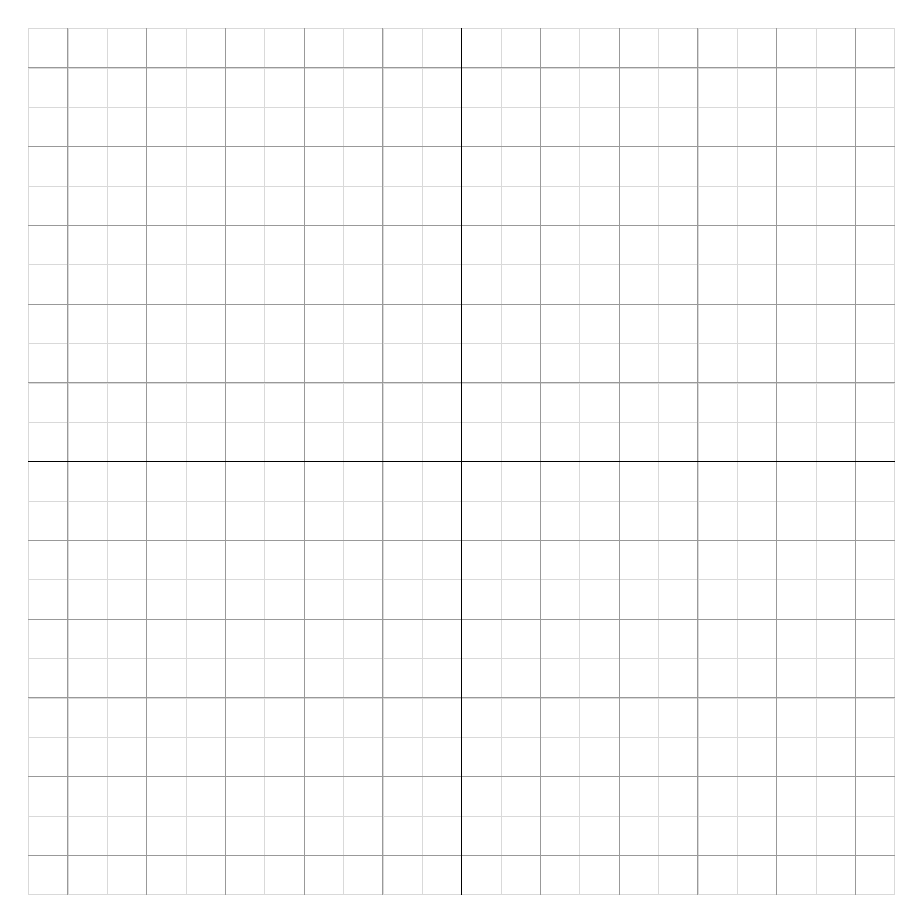
\begin{tikzpicture}
        \cartgrid{-5.5}{5.5}{-5.5}{5.5}
        \draw[axis] (-5.5,0) -- (5.5,0);
        \draw[axis] (0,-5.5) -- (0,5.5);
    \end{tikzpicture}

    \vspace*{1.2cm}

    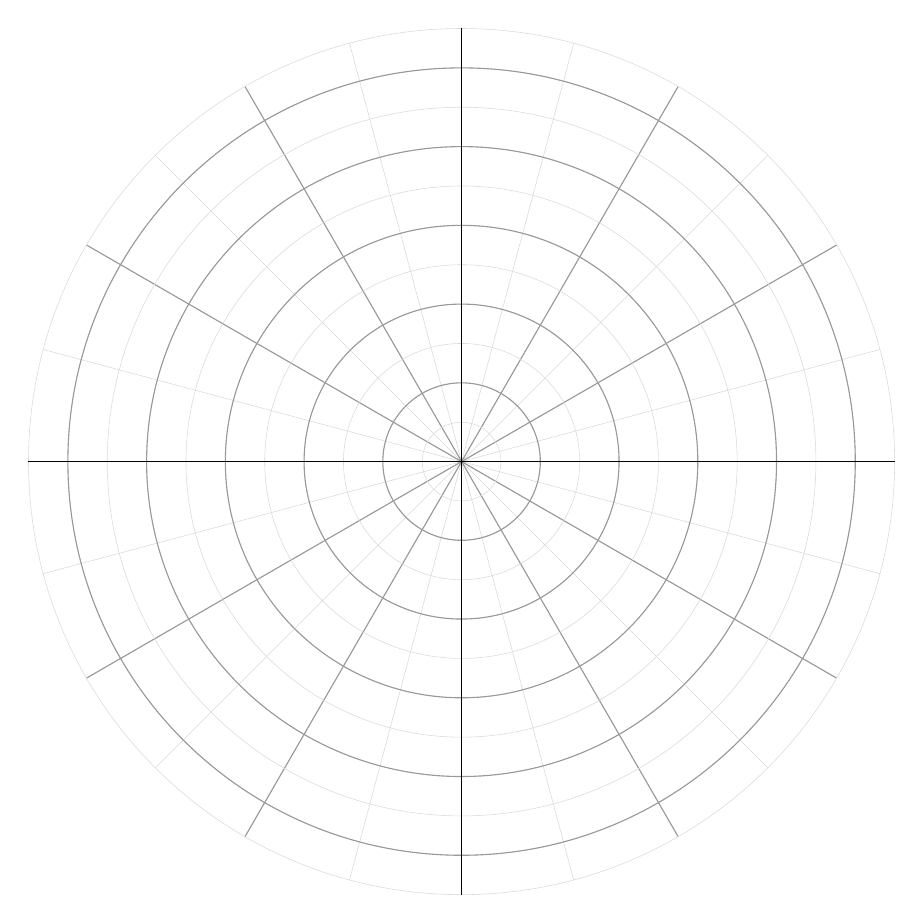
\begin{tikzpicture}
        \polargrid{5.5}{0}{360}
        \draw[axis] (-5.5,0) -- (5.5,0);
        \draw[axis] (0,-5.5) -- (0,5.5);
        \fill (0,0) circle (0.5pt);
    \end{tikzpicture}
\end{center}

\vspace*{\fill}

\newpage

% Page 2: First quadrant

\vspace*{\fill}

\begin{center}
    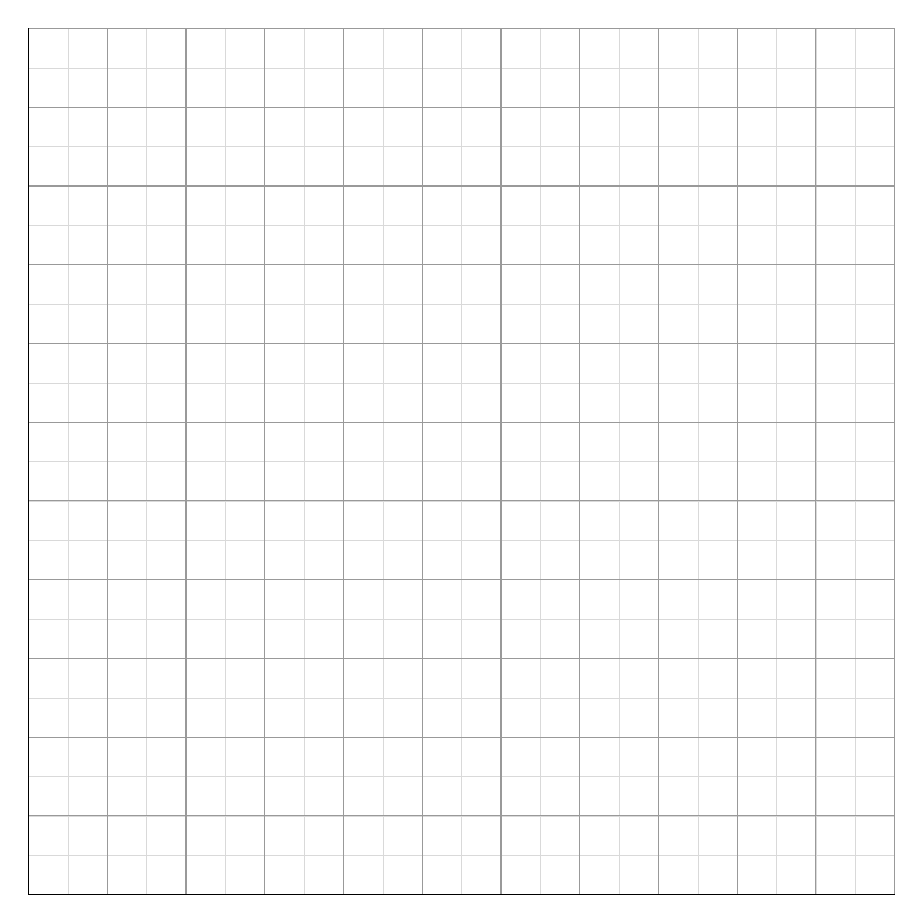
\begin{tikzpicture}
        \cartgrid{0}{11}{0}{11}
        \draw[axis] (0,0) -- (11,0);
        \draw[axis] (0,0) -- (0,11);
    \end{tikzpicture}

    \vspace*{1.2cm}

    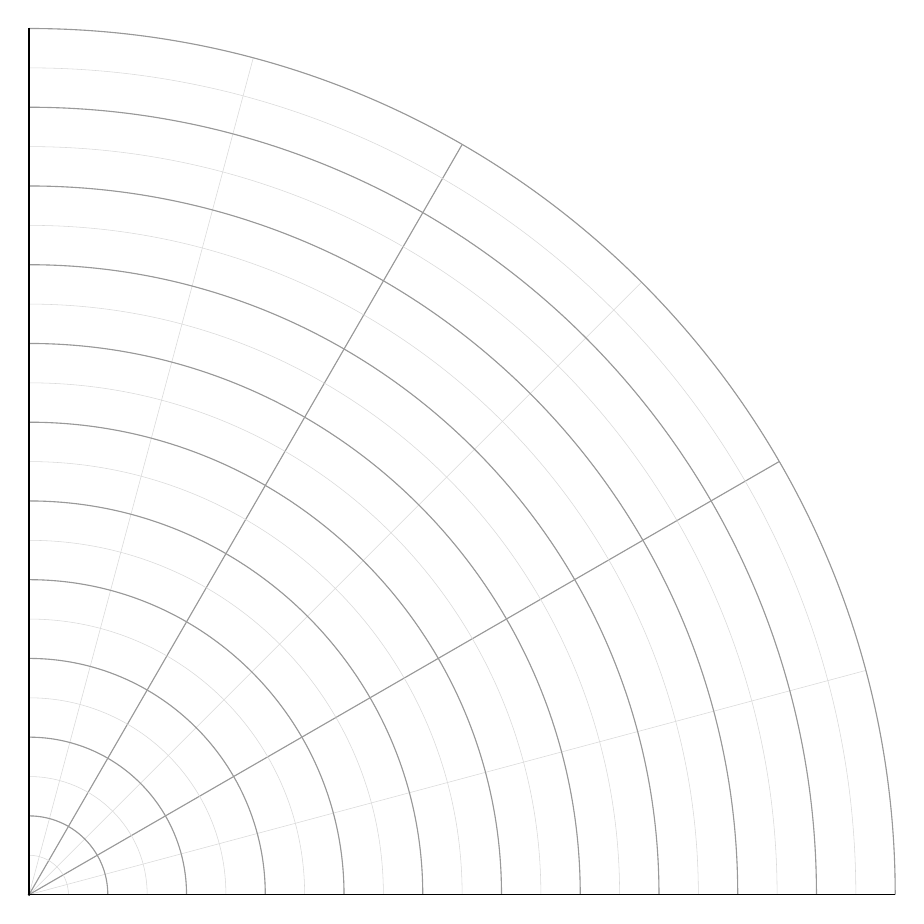
\begin{tikzpicture}
        \polargrid{11}{0}{90}
        \draw[axis] (0,0) -- (11,0);
        \draw[axis] (0,0) -- (0,11);
        \fill (0,0) circle (0.5pt);
    \end{tikzpicture}
\end{center}

\vspace*{\fill}

\newpage

% Page 3: Right half-plane

\vspace*{\fill}

\begin{center}
    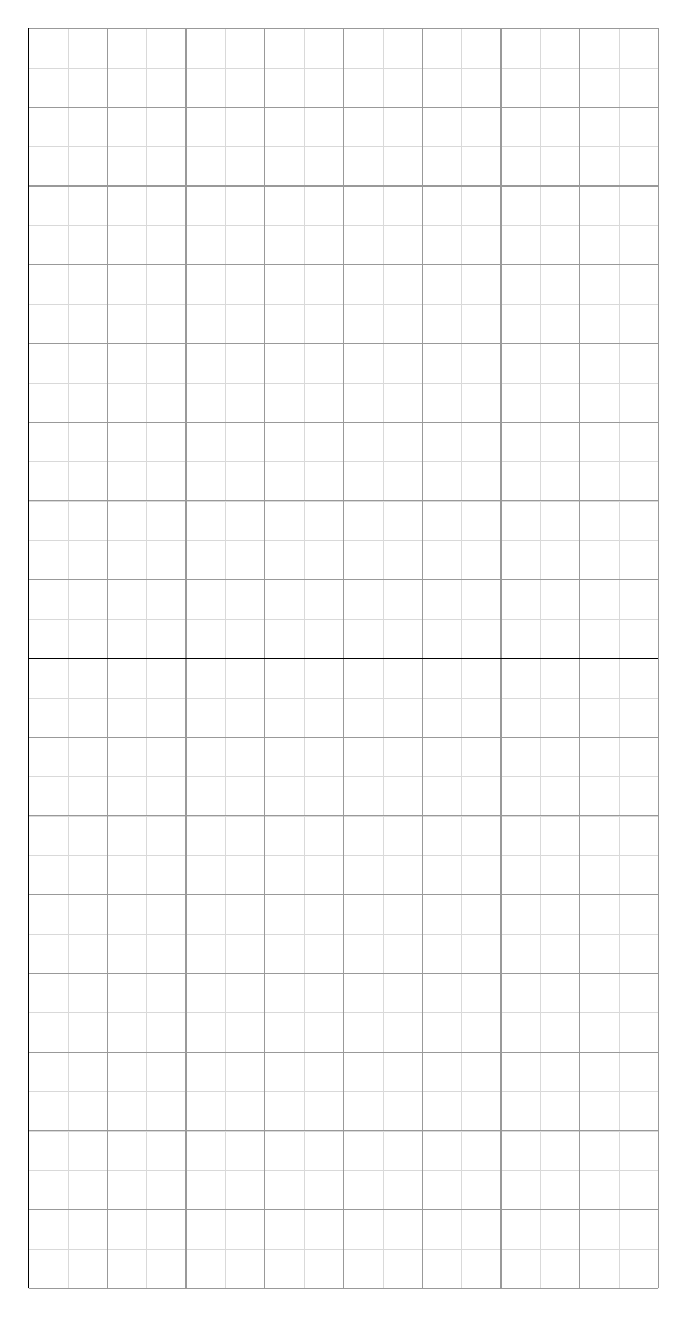
\begin{tikzpicture}
        \cartgrid{0}{8}{-8}{8}
        \draw[axis] (0,0) -- (8,0);
        \draw[axis] (0,-8) -- (0,8);
    \end{tikzpicture}
    \hspace{1.5cm}
    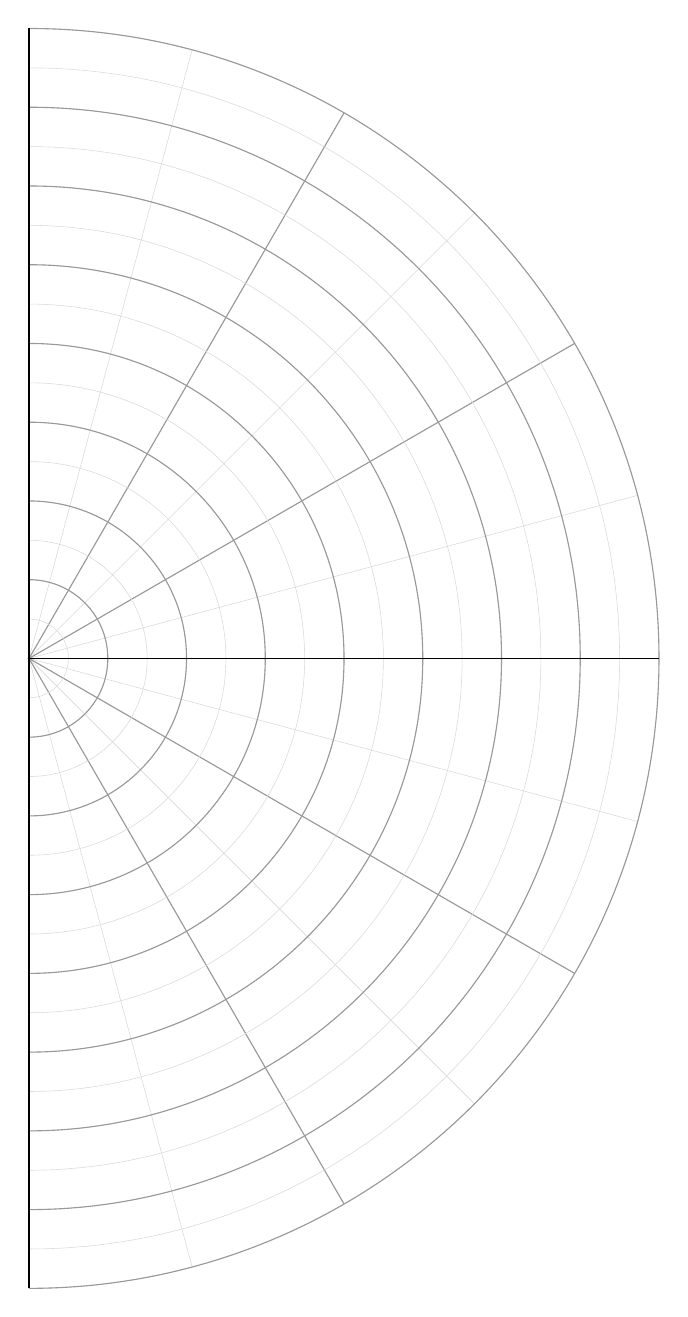
\begin{tikzpicture}
        \polargrid{8}{-90}{90}
        \draw[axis] (0,0) -- (8,0);
        \draw[axis] (0,-8) -- (0,8);
        \fill (0,0) circle (0.5pt);
    \end{tikzpicture}
\end{center}

\vspace*{\fill}

\newpage

% Page 4: Upper half-plane

\vspace*{\fill}

\begin{center}
    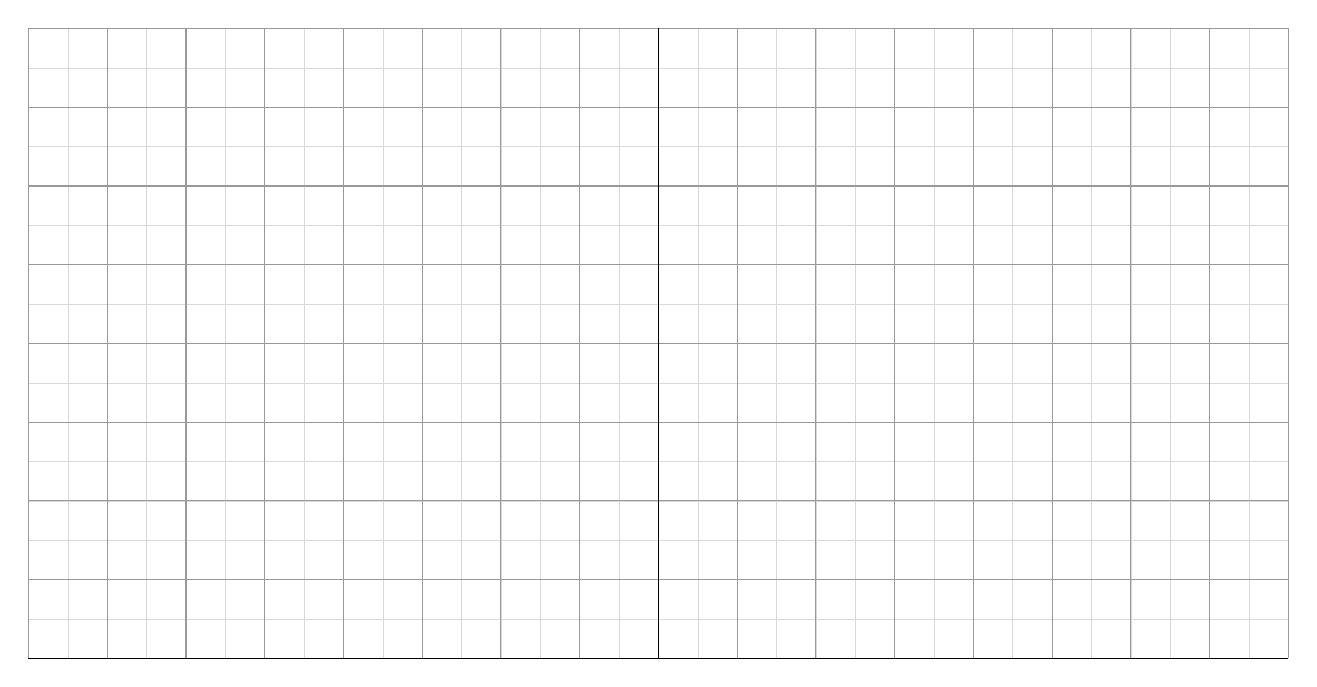
\begin{tikzpicture}
        \cartgrid{-8}{8}{0}{8}
        \draw[axis] (-8,0) -- (8,0);
        \draw[axis] (0,0) -- (0,8);
    \end{tikzpicture}

    \vspace*{1.5cm}

    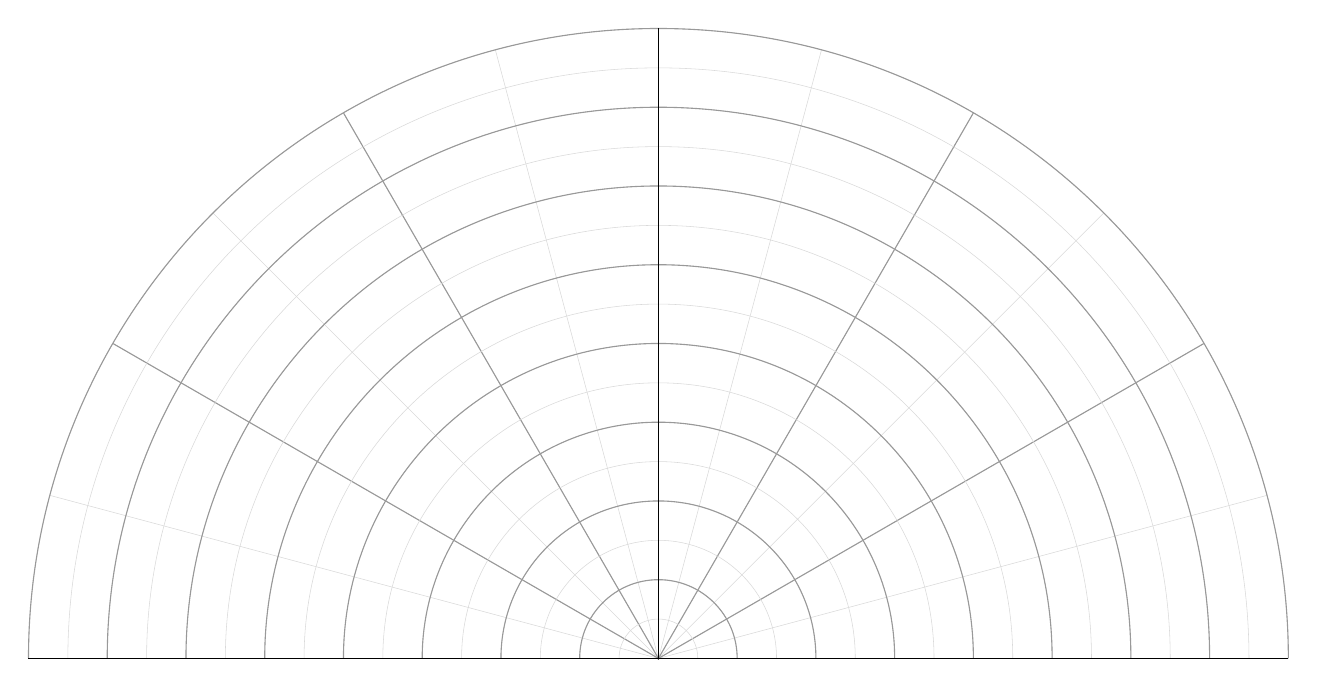
\begin{tikzpicture}
        \polargrid{8}{0}{180}
        \draw[axis] (-8,0) -- (8,0);
        \draw[axis] (0,0) -- (0,8);
        \fill (0,0) circle (0.5pt);
    \end{tikzpicture}
\end{center}

\vspace*{\fill}

\end{document}
